\chapter{Measurement Classes and Measurement Models}

\chapauthor{Stephen P. Hughes}{NASA/Goddard Space Flight Center}
\chapauthor{Darrel J. Conway}{Thinking Systems, Inc.}
\chapauthor{Matthew P. Wilkins}{Schafer Corporation}

The Measurement classes define the interfaces used to work with measurement data during the estimation process.  These classes provide access to the observation data, typically provided by way of a data file, using a helper object derived from the MeasurementReader base class.  The Measurement classes provide methods that calculate the expected value of a specific measurement type, along with the derivative data needed for estimation.  These data include calculation of expected measurements, measurement partials, determination of measurement feasibility, and interactions with root finders to determine tracking schedules and light time corrections.  A measurement object acts as a participant in the measurement, as the measurement object contains estimated states associated with measurement errors.

The measurement hierarchy consists of a base class and a tiered hierarchy of derived classes as shown in Figure~\ref{fig:MeasurementClasses}.  The following sections discuss each class in the hierarchy in detail, starting with the Measurement base class.

\begin{figure}[htbp]
\begin{center}
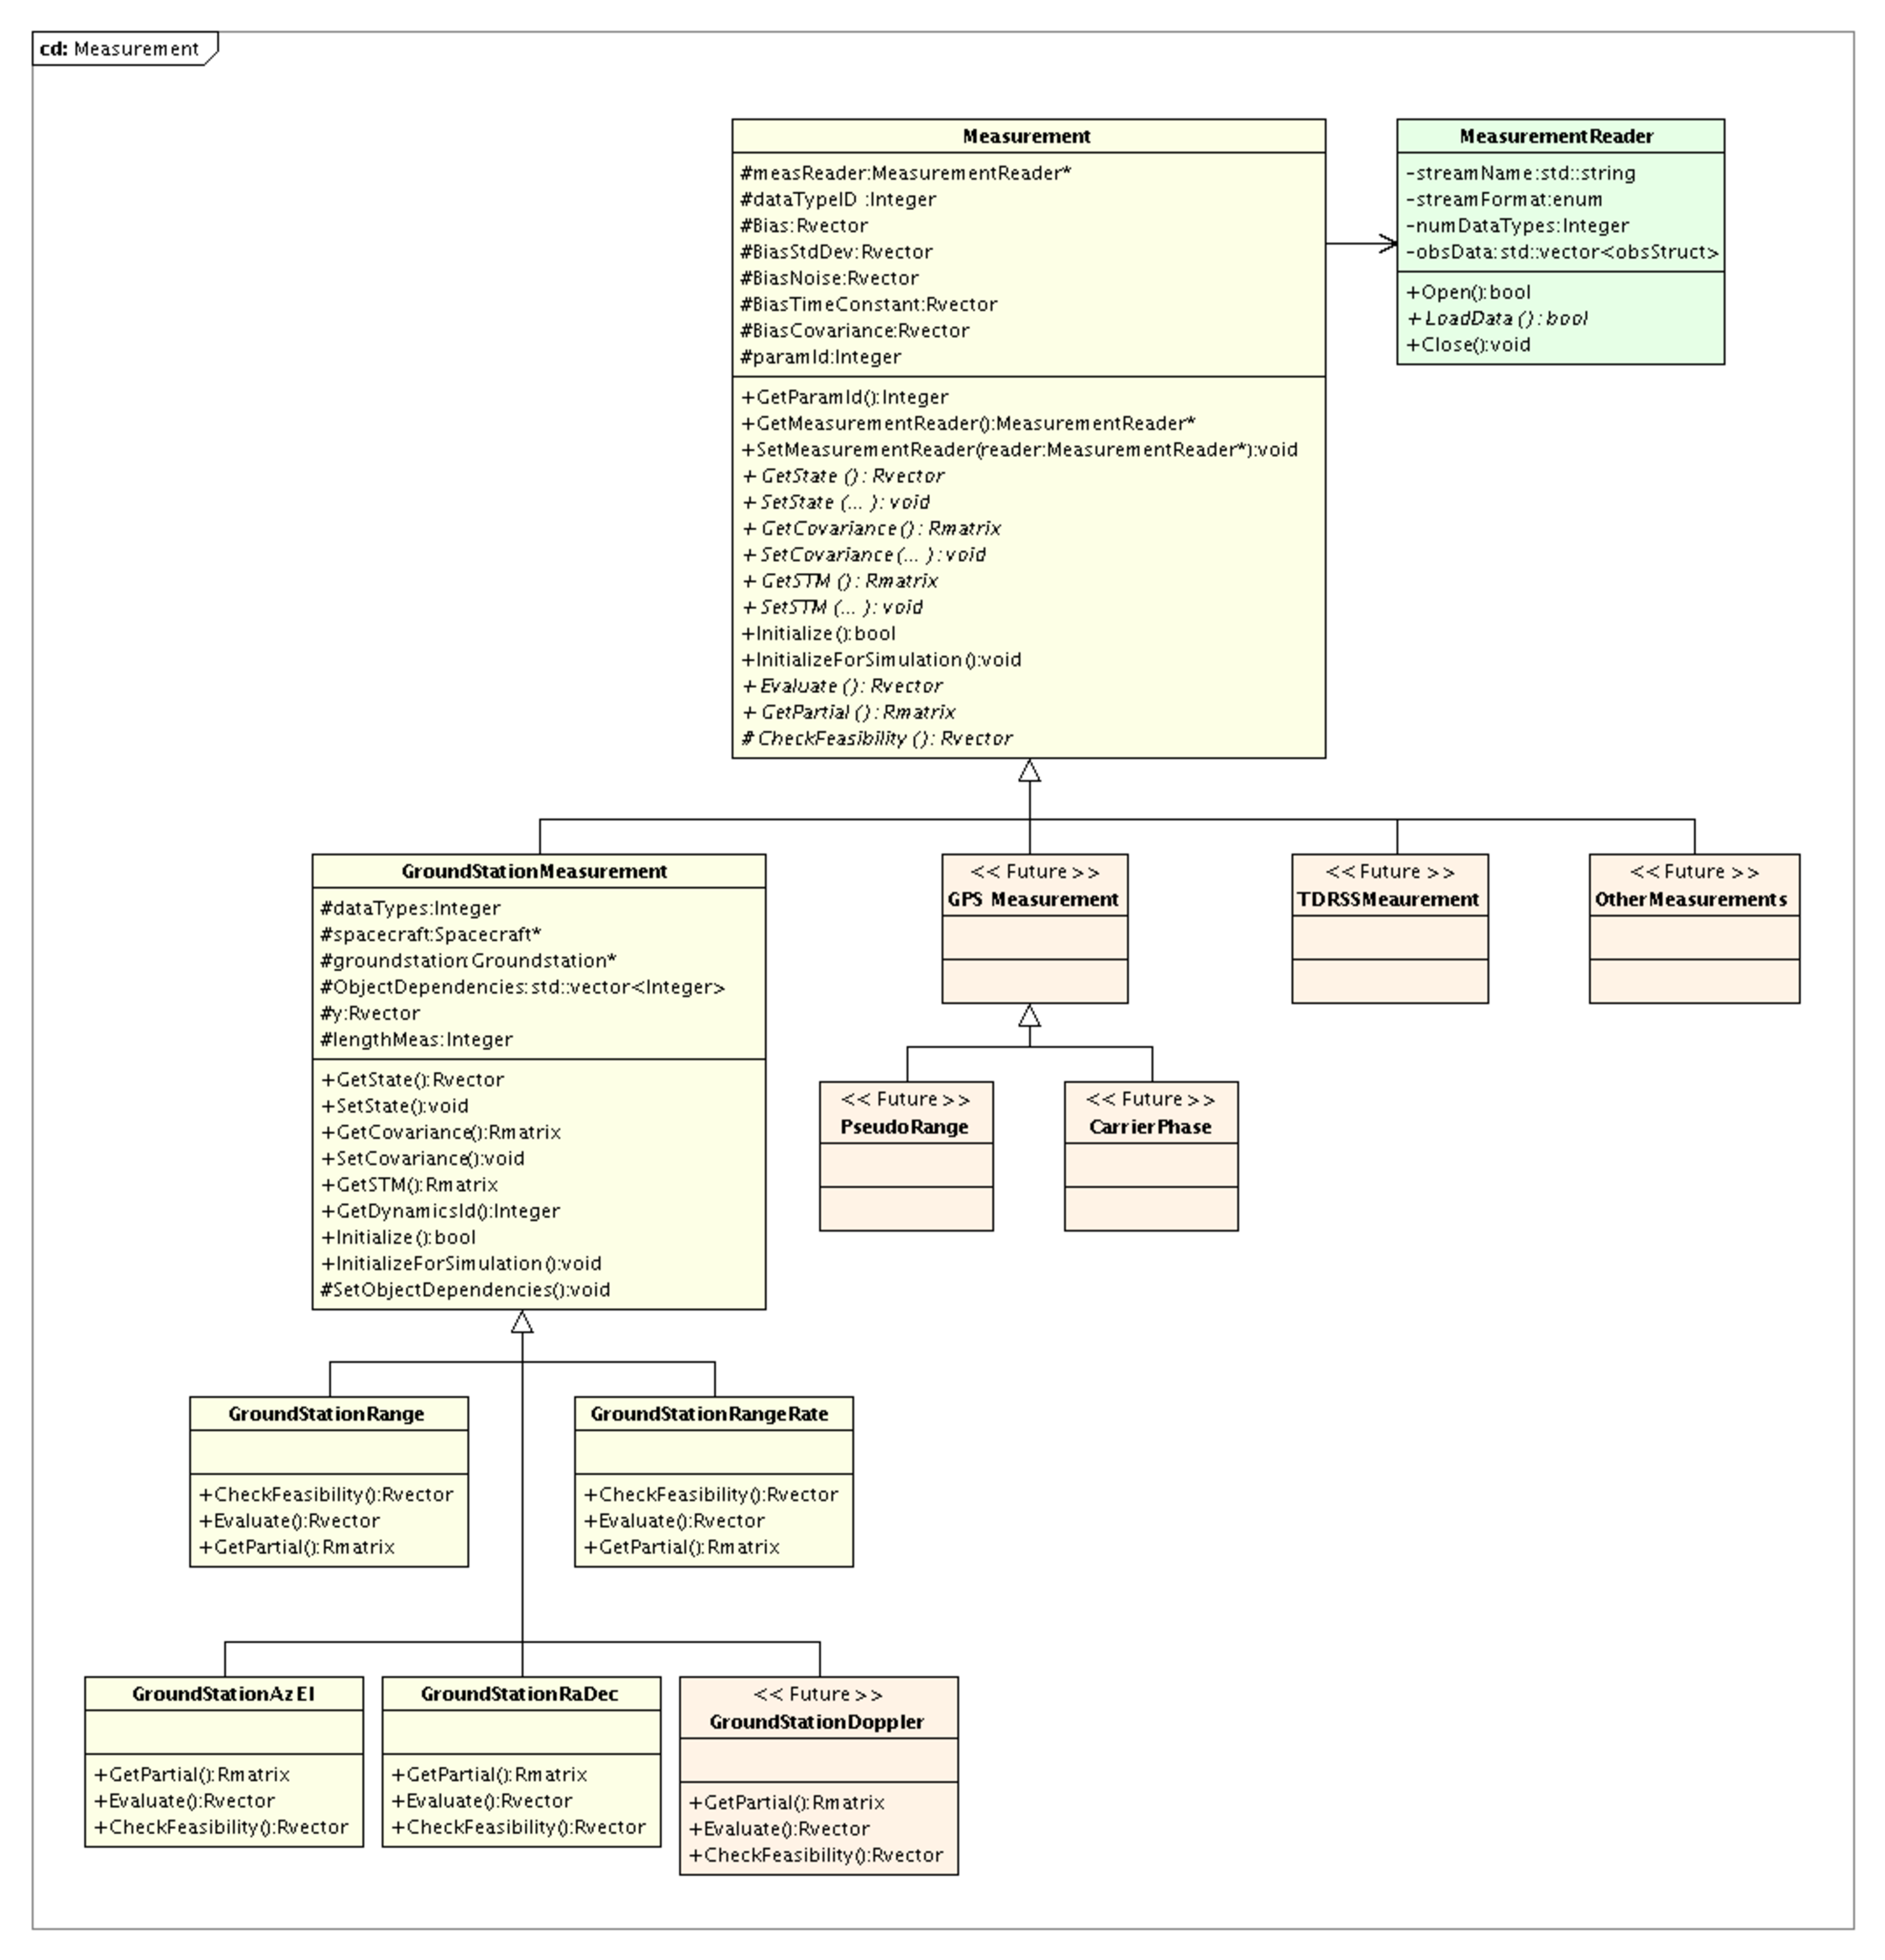
\includegraphics[scale=0.43]{Images/MeasurementClasses.eps}
% MeasurementClasses.png: 1061x1104 pixel, 72dpi, 37.43x38.95 cm, bb=0 0 1061 1104
\caption{\label{fig:MeasurementClasses}The Measurement Class Hierarchy}
\end{center}
\end{figure}

\section{The Measurement Class}

The Measurement base class contains member data and functions associated with all measurement objects as well as data associated with parameters that are set by the user when configuring the measurement object.  Examples of these data include the measurement file name and format, the data types to be processed from the file, and measurement stochastic properties such as biases and time constants.

The Measurement class defines many of the interfaces implemented in the derived classes so that the estimation process can work with measurement objects using base class references and pointers.  These interfaces are defined as either overridable or abstract (that is, pure virtual) methods on the Measurement base class.  The derived classes implement custom versions of these methods that are specific to the measurement type being implemented.  The data members of the Measurement base class are described below, followed by descriptions of the methods provided in the Measurement base class.  Finally, we will describe the MeasurementReader helper class before moving to the definitions of the derived classes.

\subsection{Measurement Members}

\paragraph{Member Attributes}

The list below describes the data elements provided in the Measurement base class to support the derived classes.  These elements are designed to facilitate access to measurement information through calls to a Measurement instance pointer.  Some Measurement objects provide multiple data elements.  For that reason, some of the data members listed here gain a dimension over what might be expected for single-valued measurements.  For example, the ground station RA/Dec measurement type returns two values for each measurement: the right ascension and declination values, so the methods that calculate these values return an Rvector rather than a Real number.  Since there are
Measurement classes that have this multivalued return requirement, GMAT uses an Rvector for the data, even when the return value is a single number.

The data members of the Measurement are:

\begin{itemize}
\item \textbf{MeasurementReader *measReader}:  The MeasurementReader that supplies the observation data. This pointer can be NULL when simulating data.
\item \textbf{Integer dataTypeID}:   An integer containing the Id for the data type.  Although the user may specify several data types on a measurement object, GMAT creates an object for each data type during initialization.  Each object has an Id associated with its data type which is specified by dataTypeId.
\item \textbf{Rvector Bias}:  A vector of real numbers containing the measurement biases.  These data can be estimation state parameters.
\item \textbf{Rvector BiasStdDev}:  A vector of real numbers containing the standard deviations of the biases. These data can be estimation state parameters.
\item \textbf{Rvector BiasNoise}:  A vector of real numbers containing the noise in the measurement biases. These data can be estimation state parameters.
\item \textbf{Rvector BiasTimeConstant}:  A vector of real numbers containing the time constants for the measurement biases. These data can be estimation state parameters.
\item \textbf{Rvector BiasCovariance}:  A vector of real numbers containing the bias covariances.
\item \textbf{Integer ParamId}:  ID for the type of measurement parameter?
\item \textbf{Integer numDataTypes}:  The number of data types the user specified on the measurement object. During measurement initialization, a new object is created for each data type specified on the measurement object.
\end{itemize}

\paragraph{Class Methods}

The Measurement class includes the following methods designed to make access to measurement data as generic as possible by the classes that use Measurement objects.  Many of these methods are abstract (pure virtual in C++ terminology): they are defined in this base class, but no implementation is provided in the base class.  The abstract classes can be identified by an ``= 0'' suffix in this list.

\begin{itemize}
\item \textbf{enum MeasurementFormat}: An enumeration defining the supported measurement formats.  Note: This enumeration is not a class member; it is a member of the Gmat namespace.
\item \textbf{Integer GetParameterId()}: A method to determine the integer id for solve-for and consider parameters on the measurement object.  This is how the system converts from the string definition provide by the user, say MauiGSRange.Bias,to a numeric Id.  <DJC: Not sure of this part.>
\item \textbf{MeasurementReader *GetMeasurementReader()}:  Retrieves a pointer to the
MeasurementReader.
\item \textbf{void SetMeasurementReader(MeasurementReader *reader)}:  Sets the pointer to the MeasurementReader.
\item \textbf{virtual Rvector\& GetState() = 0}: Retrieves the state vector.
\item \textbf{virtual void SetState(Rvector\& newState) = 0}:  Sets the state vector to match the provided data.
\item \textbf{virtual Rmatrix\& GetCovariance()= 0}:  Retrieves the covariance matrix.
\item \textbf{virtual void SetCovariance(Rmatrix\& newCovariance) = 0}:  Sets the covariance matrix data.
\item \textbf{virtual Rmatrix\& GetSTM() = 0}: Retrieves the state transition matrix.
\item \textbf{virtual void SetSTM(Rmatrix\& newSTM) = 0}: Sets the STM matrix data.
\item \textbf{virtual bool Initialize()}: Prepares the Measurement object for use in a Sandbox.
\item \textbf{virtual void InitializeForSimulation()}:  Prepares the Measurement object for use during measurement simulation.
\item \textbf{virtual Rvector\& Evaluate() = 0}:  Calculates the expected observation value.
\item \textbf{virtual Rmatrix\& GetPartial() = 0}:  Retrieves the measurement partial derivative matrix.
\item \textbf{virtual Rvector\& CheckFeasibility() = 0}:  Checks to see if a measurement can be made using the current state information.
\end{itemize}

\section{GroundstationMeasurement}

Measurements that are made at a ground station are modeled using the GroundStationMeasurement class.  Data and member functions that are common to all Ground Station measurements are located on the GroundStationMeasurement class, including the participants in the measurement process, Get/Set functions, and common modeling algorithms.   Below we discuss in detail all member data and functions.

\subsection{GroundstationMeasurement Members}

\paragraph{GroundStationMeasurent Attributes}

\begin{itemize}
\item \textbf{Integer dataTypes}:  ???
\item \textbf{Spacecraft *spacecraft}:  A pointer to the spacecraft that is participating in the measurement. This pointer is set during measurement initialization.
\item \textbf{Groundstation *groundstation}:  A pointer to the ground station that is participating in the measurement.  This pointer is set during measurement initialization.
\item \textbf{std::vector<Integer> ObjectDependencies}: A vector of integers that contains information on how participants on a measurement object map to participants in the overall estimation problem.  In general, the participants on a measurement are a subset of the participants for the estimation problem.  The ObjectDependencies is used primarily to determine partial derivatives and ensure they are placed in the correct location in the overall partial derivative array.  The ESM maintains an array of pointers, called ObjectsVector, to the participant associated with each state chunk in the estimation problem.  The ObjectDependencies array is the same length as ObjectsVector.  If, for example, element 1 of ObjectDependencies is zero, then the first object in the estimator's participant list is not a participant in the measurement.  If element 1 is nonzero, then the integer is associated with the participant Id used internally by the measurement.  The ObjectDependencies array is set during initialization when the Measurement Manager makes a call to initialize the measurement.
\item \textbf{Rvector y}:  The vector of calculated measurements.
\item \textbf{Integer lengthMeas}:  ???
\end{itemize}

\paragraph{}GroundStationMeasurement Methods:

\begin{itemize}
\item \textbf{SetState}:  Given a state value and id, this method updates the state on the measurement object.
\item \textbf{GetState}:  Given a state id, this method gets the state from the measurement object.
\item SetCovariance:  Given a covariance matrix and the state id, this method updates the state's covariance on the measurement object.
\item \textbf{GetCovariance}:  Given a state id, this method gets the state's covariance from the measurement object.
\item \textbf{GetSTM}: Given a state id, this method gets the states' STM.
\item \textbf{GetDynamicsId}:  Given a state Id, this method returns the ODE model ID for use in propagation of the state and it's STM.  Not implemented yet for measurement.
\item \textbf{Initialize}:  This method makes a call to the file reader and gets the observations and epochs from the requested data type.  If there are multiple data types on the measurement, the measurement object concatenates them into the Obs and Epochs Arrays.  These are then extracted by the measurement manager later in the initialization process.     For each data type, a new object is created and pointers to the object's participants are set.  (Matlab currently only supports one data type per measurement.  Not a difficult mod though)
\item \textbf{InitializeforSimulation}:  This method prepares a measurement object for simulation.  The process is similar to the Initialize method on GroundStationMeasurement, with the exception the reading and managing observations and epochs is not required.
\item \textbf{GetDataTypeId}:  This method returns the integer Id for the measurement type, given the string name for the measurement.
\item \textbf{SetObjectDependencies}:  This method takes as input an array of pointers to the participants in the estimation state vector.   The method steps through each element in the input array and determines if it points to any of the measurement participants.   If not, then the element in ObjectDependencies is set to zero.  If so, then the element is set to the Id of the participant used internally by the measurement object.
\end{itemize}

\section{GroundStationRange}

The GroundStationRange class is derived from the GroundStationMeasurement class, and performs modelling range measurements, measurement feasibility, and partial derivatives, and light time iteration.

\subsection{GroundstationRange Members}

\paragraph{GroundStationRange Attributes}

None.  The data members in the GroundStationMeasurement class are sufficient for this class.

\paragraph{GroundStationRange Methods}

\begin{itemize}
\item \textbf{CheckFeasibility}:  This method evaluates the feasibility function for the range measurement. If the value of the feasibility function is positive, then the conditions required to perform a measurement are met.  If the feasibility function is negative, conditions are not met.  Event locators determine the roots of the feasibility function to determine tracking data scheduling.
\item \textbf{Evaluate}:  The evaluate function calculate the computed value of the measurement based on the current state of the participants.
\item \textbf{GetPartial}:  This method returns the requested partial derivative based given a participant Id and the state Id.  The participant Ids are contained in the array ObjectDependencies.  This method is called by the measurement manager to determine individual partials. The measurement manager assembles the entire partial derivative from the pieces returned by the measurement object.
\end{itemize}

\section{The MeasurementManager Class}

The measurement manager functions as the interface between the Estimator and the measurement objects
defined by the user.  The primary jobs of the measurement manager are

\begin{itemize}
\item To coordinate measurement data and provide observed and computed values to the estimator
\item To maintain the sorted list of observed measurement quantities from all measurement sources.
\item To assemble the H matrix for each measurement based on state information and the partials map
provided by the measurements.
\end{itemize}
